\documentclass{article}
\usepackage{natbib}
\usepackage{graphicx}
\usepackage{csquotes}
\usepackage{hyperref}
\usepackage{booktabs}
\usepackage{multirow}
\usepackage[table]{xcolor} 
\usepackage{graphicx}
\usepackage{caption}
\usepackage{amsmath}
\usepackage[margin=4cm]{geometry}

%---------------------------------- NATBIB ----------------------------------%
\makeatletter
% natbib: only make year a hyperref, not author
\let\oldciteauthor\citeauthor

\def\citeauthor#1{{\NoHyper\oldciteauthor{#1}}}

% Patch case where name and year are separated by aysep
\patchcmd{\NAT@citex}
  {\@citea\NAT@hyper@{%
     \NAT@nmfmt{\NAT@nm}%
     \hyper@natlinkbreak{\NAT@aysep\NAT@spacechar}{\@citeb\@extra@b@citeb}%
     \NAT@date}}
  {\@citea\NAT@nmfmt{\NAT@nm}%
   \NAT@aysep\NAT@spacechar\NAT@hyper@{\NAT@date}}{}{}

% Patch case where name and year are separated by opening bracket
\patchcmd{\NAT@citex}
  {\@citea\NAT@hyper@{%
     \NAT@nmfmt{\NAT@nm}%
     \hyper@natlinkbreak{\NAT@spacechar\NAT@@open\if*#1*\else#1\NAT@spacechar\fi}%
       {\@citeb\@extra@b@citeb}%
     \NAT@date}}
  {\@citea\NAT@nmfmt{\NAT@nm}%
   \NAT@spacechar\NAT@@open\if*#1*\else#1\NAT@spacechar\fi\NAT@hyper@{\NAT@date}}
  {}{}
  
\makeatother
%-------------------------------------------------------------------------------%


%----------------------------------- HREF ------------------------------------%
% define href colors
\hypersetup{
    colorlinks=true,
    linkcolor=blue,
    filecolor=blue,      
    urlcolor=blue,
    citecolor=blue
}
\urlstyle{same}
%-------------------------------------------------------------------------------%


\begin{document}
\graphicspath{ {../../../output/03-results/plots/} }

\section{What Has to be Mentioned Before}
\label{sec:before}

\section{Data}

The data for this study comprises two distinct corpora: a corpus with legal documents and a baseline corpus with comments from Reddit, the world's largest online-forum. The legal corpus contains court opinions from Court of Appeals for 1st to 11th circuit, based on open data provided by the \citet{FreeLawProject2020}. For the baseline corpus, we gathered data using the API for the Pushshift Reddit Data Set provided by \citet{Baumgartner2020}. 

In our case, the corpus generation is an iterative process. We start off with a list of target adjectives we specified without information about the corpora. This initial list, $L_1$, includes 2x5 adjectives that often discussed by the TC-literature and we deem rather uncontroversial. The list contains epistemic concepts (XXX), thick (XXX) concepts (XXX) as well as legal concepts (XXX). However, some of these adjectives are rarely used in the legal context, while others may occur frequently, yet are most often part of legal phrases, which indicate a different semantic embedding. In order to avoid any sort of selection bias and exclude adjectives with predominantly phrasal use, we inductively select a second battery of adjectives. This inductive approach is based on an analysis of part of speech (PoS)-sequences in the legal corpus. PoS-tagging is an unsupervised method to annotate the syntactic structure of text data. For each of the subcorpora (1st to 11th Court of Appeals), we first draw a random sample of 2000 documents which are subsequently PoS-tagged using UDPipe \citep{Straka2017, Straka2020}. Based on these PoS-tags, we isolate all syntactic structures of the form $(M)*A(,)*C(M)*A$ (M = modifier, A = adjective, C = conjunction, (...) = optional part). The conjuncts are then pooled across all subcorpora and only AND-conjunctions are retained. Finally, all adjectives %$A_i...A_n$ 
are ranked according to frequency as well lexical diversity in regards to the conjoined adjectives. We use Yule's \textit{K} \citep{Yule1944, Tweedie1998} as a measure for lexical diversity.  %In addition, we map them on a dissociation dimension, which gives a measure of how exclusive the set of conjoined adjectives is for a specific $A_i$.
Based on this ranking, we manually select adjectives that match our concept classes and add antonyms to form list $L_2$. In a third step, we combine $L_1$ and $L_2$, and use them to retrieve documents containing suitable target structures both from the legal corpus and via the Pushshift API. In a last step, we determine the three most promising concepts per class, based on number of occurences and Yule's $K$, and reduce the respective corpora accordingly. The final list of adjectives is shown in \ref{tab:l3} in the \ref{sec:appendix}. 

The full legal corpus has XXX entries, the baseline corpus XXX. In order to keep the computational resources low while keeping a high enough $n$, we reduce the legal subcorpora each randomly by -40\%, resulting in XXX legal documents overall. Both corpora are subsequently cleaned, PoS-tagged, lemmatized and the conjoined adjectives are annotated with sentiment values from the SentiWords dictionary based on SENTIWORDNET \citep{Esuli2006, Baccianella2010, Guerini2013, Gatti2016}.

\section{Method}

In the following, we will discuss the methods used in our two studies.

\subsection{Study 1}

In the first study, we assess the average context effects for both corpora. First, we estimate the average sentiment intensity of conjoined adjectives in each corpus. The basis for this analysis is a linear model with the absolute conjoined sentiment values as dependent and the corpus-dummy as independent variable. Based on this model, we compute the estimated marginal means for the corpora. This gives on overall estimate of differences in sentiment intensity between the corpora, irrespective of polarity. 

The second model further discriminates between positive and negative target adjectives, but does not yet include the concept classes. Instead of using absolute sentiment values as dependent variable, this model uses the non-transformed values. The polarity-discriminator is added as an interaction term between the corpus-dummy and the polarity-dummy for the target adjectives. This allows us to assess the estimated marginal means of the conjoined sentiment values for each corpus by target polarity.

The third and final model estimates the differences between corpora for each concept class. Because we are mostly interested in differences in terms of intensity, the model once again uses absolute conjoined sentiment values. As estimator we use an interaction term between the corpus dummy and the concept class factor.

\subsection{Study 2}

In the second study, we focus on the legal corpus only. In order to be able to compare the results of the evaluative concepts classes to a baseline, we added corpus entries for the following descriptive target adjectives: XXX. Instead of comparing context effects (Study 1), we want to inquire whether the concept classes cluster differently within the legal context. We use a combination of K-Means Clustering and Principal Component Analysis (PCA), which is informed by the sentiment values of the conjoined adjectives and a measure for lexical diversity of the target adjective, i.e. Yule's \textit{K} \citep{Yule1944, Tweedie1998}. The cluster analysis further includes information based on the vector space of the corpus, which is created using the \textit{Semantic Vectors} package \citep{Widdows2008, Widdows2010, Widdows2016}. For every pair of target adjective and conjoined adjective, we compute the cosine similarities. Cosine similarities are essentially high dimensional representations of co-occurence measures, and inform the cluster analysis about the semantic similarity of the conjuncts by taking the whole corpus into account. In the final ANOVA model, the cosine similarities are added as weights for the sentiment values of the conjoined adjectives.

\section{Results}

Before we move to the results of our studies, there will be a brief discussion of the summary statistics of the text data.

\subsection{Descriptive Statistics}

The summary statistics are split by corpus. Table \ref{tab:LCstats} shows the measures of sentiment dispersion and lexical diversity by class and polarity for the legal corpus (LC). Table \ref{tab:BCstats} contains the same for the baseline corpus (BC). 

The sentiment dispersion in Table \ref{tab:LCstats} indicates more extreme values for negative target adjectives overall. According to Yule's \textit{K}, their conjuncts are also more lexically diverse than the ones of the positive target adjectives. The average observed sentiment is consistent with our assumption that AND-conjunctions pair adjectives of the same polarity. The descriptive concept have a very neutral average (0.02), which is also consistent with our expectations. However, there seems to be an overlap between descriptive concepts several concept classes, which might prove to be significant later on.

\begin{table}[ht]
\centering
\rowcolors{5}{gray!25}{white}
\begin{tabular}{rlrrrrrrrr}
  & & \multicolumn{3}{c}{Sentiment Quantiles} & & \multicolumn{3}{c}{Lex. Diversity}\\
   \cmidrule{3-5} \cmidrule{7-9}
  Class & Polarity & 25\% & 50\% & 75\% & Avg. &  TTR & CTTR & K\\
  \bottomrule
Descriptive & neutral & -0.18 & 0.00 & 0.22 & 0.02 & 0.15 & 6.17 & 168.36 \\ 
  Epistemic & negative & -0.44 & -0.33 & -0.10 & -0.26 & 0.16 & 6.09 & 124.78 \\ 
  Epistemic & positive & 0.04 & 0.14 & 0.30 & 0.17 & 0.05 & 3.68 & 342.11 \\ 
  Legal & negative & -0.40 & -0.29 & 0.00 & -0.19 & 0.13 & 4.69 & 249.80 \\ 
  Legal & positive & 0.07 & 0.22 & 0.22 & 0.17 & 0.04 & 2.93 & 1530.47 \\ 
  TC & negative & -0.44 & -0.35 & -0.20 & -0.30 & 0.11 & 4.81 & 507.77 \\ 
  TC & positive & 0.06 & 0.16 & 0.33 & 0.21 & 0.06 & 3.55 & 640.33 \\ 
   \hline
\end{tabular}
\caption{Summary Statistics LC}
\label{tab:LCstats}
\end{table}

Table \ref{tab:BCstats} indicates a far more polar sentiment dispersion in BC compared to LC, which is also reflected by the more polar averages. Lexical diversity is a lot higher in BC than LC, which was to be expected, due to the more codified nature of legal language use. The difference in homogeneity is most acute for legal concepts and TC, and less so for epistemic concepts.

\begin{table}[ht]
\centering
\rowcolors{5}{gray!25}{white}
\begin{tabular}{rlrrrrrrrr}
  & & \multicolumn{3}{c}{Sentiment Quantiles} & & \multicolumn{3}{c}{Lex. Diversity}\\
   \cmidrule{3-5} \cmidrule{7-9}
  Class & Polarity & 25\% & 50\% & 75\% & Avg. &  TTR & CTTR & K\\
  \bottomrule
Epistemic & negative & -0.52 & -0.42 & -0.18 & -0.34 & 0.10 & 7.65 & 73.19 \\ 
  Epistemic & positive & 0.16 & 0.29 & 0.50 & 0.30 & 0.08 & 7.26 & 94.69 \\ 
  Legal & negative & -0.55 & -0.44 & -0.24 & -0.38 & 0.13 & 6.65 & 198.62 \\ 
  Legal & positive & 0.00 & 0.22 & 0.45 & 0.21 & 0.09 & 6.43 & 132.81 \\ 
  TC & negative & -0.55 & -0.45 & -0.29 & -0.39 & 0.09 & 6.93 & 80.10 \\ 
  TC & positive & 0.16 & 0.32 & 0.52 & 0.31 & 0.09 & 7.06 & 125.27 \\ 
   \hline
\end{tabular}
   \caption{Summary Statistics BC}
   \label{tab:BCstats}
\end{table}

The sentiment dispersion on the level of the target adjectives are shown in Figure \ref{fig:SDta}. As we can see, the polarity of the target adjective is a good indicator for the polarity of the conjoined adjective, and vice versa. With the exception of \textit{lawful} and \textit{unlawful}, the sentiment spread is mostly limited to either the positive or the negative region of the scale and does not include the midpoint. The differences between the corpora also become apparent on the level of the target adjectives: LC has lower averages (i.e. dots) than BC across the board, with the exception of \textit{dishonest} and \textit{improper}. This becomes even more apparent on when aggregated by class (i.e. horizontal lines).

\begin{figure}[ht]
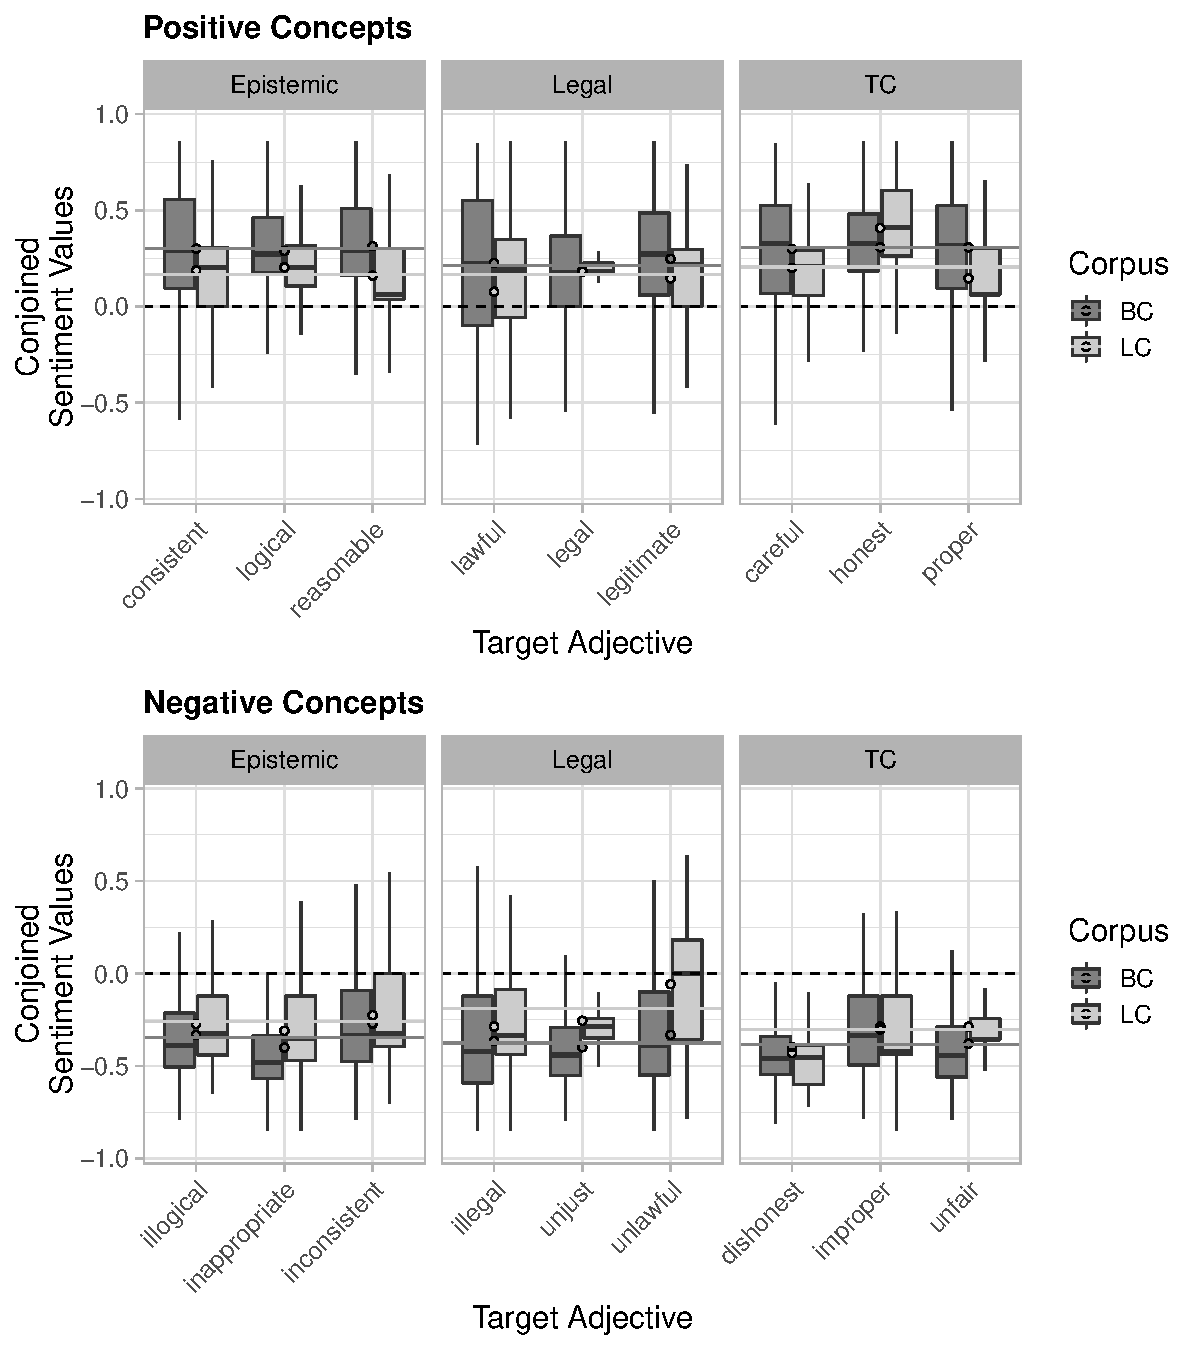
\includegraphics[width=\textwidth, keepaspectratio]{bc_lc_summary_stats_adj-distr}
\caption{Sentiment Dispersion by Target Adjective}
\label{fig:SDta}
\end{figure}


\subsection{Study 1}

The first model of study 1 is presented in Table \ref{tab:s1m1} and shows the effect of context (LC v. BC) on the absolute sentiment of conjoined adjectives. According to the linear model, LC has an average effect of $\beta = -0.1262$ compared to BC, $t\text{-value:} -99.63$, $Pr(>|t|) = <2e^{-16}$, all other things equal. The estimated marginal mean for BC is $0.3622$, the one for LC is $0.2360$. Hence, the sentiment values of the conjoined adjectives are indeed less intense for LC than for BC.

\begin{table}[ht]
\centering
\begin{tabular}{lrrrrr}
  \hline
Corpus & Est. Mean & SE & df & lower CL & upper CL \\ 
  \hline
BC & 0.3622 & 0.0008 & 109920 & 0.3607 & 0.3637 \\ 
  LC & 0.2360 & 0.0010 & 109920 & 0.2341 & 0.2380 \\ 
   \hline
\multicolumn{6}{l}{{\footnotesize Results are given on the absolute scale. Confidence level used: 0.95}}\\
\end{tabular}
\caption{Absolute Estimated Mean Sentiment Difference Between Corpora}
\label{tab:s1m1}
\end{table}

The second model shows similar results, even if we take polarity into account. The effect of positive polarity compared to negative polarity is $\beta_1 = 0.6456$, $t\text{-value:}324.43$, whereas the effect of LC compared to BC drops slightly to $\beta_2 = 0.1085$, $t\text{-value:}35.31$. The interaction of positive polarity and LC compared to the intercept has an effect of $\beta_3 = -0.2130$, $t\text{-value:}-58.68$. All effects are highly significant on a 0.05 alpha-level ($Pr(>|t|) = <2e^{-16}$). Table \ref{tab:s1m2} contains the estimated marginal means for this model. In summary, LC has significantly more neutral sentiment values than BC on both sides of the sentiment scale.

\begin{table}[ht]
\centering
\begin{tabular}{lrrrrr}
  \hline
Corpus & Est. Mean & SE & df & lower CL & upper CL \\ 
\hline
\multicolumn{6}{l}{Polarity = negative}\\
\cmidrule{1-2}
BC & -0.3659 & 0.0015 & 109918 & -0.3689 & -0.3629 \\ 
  LC & -0.2574 & 0.0027 & 109918 & -0.2627 & -0.2522 \\ 
   \cmidrule{1-6}
\multicolumn{6}{l}{Polarity = positive}\\
\cmidrule{1-2}
BC & 0.2797 & 0.0013 & 109918 & 0.2772 & 0.2822 \\ 
  LC & 0.1752 & 0.0015 & 109918 & 0.1723 & 0.1780 \\ 
   \hline
\multicolumn{6}{l}{{\footnotesize Confidence level used: 0.95}}\\
\end{tabular}
\caption{Estimated Mean Difference Between Corpora by Target Polarity}
\label{tab:s1m2}
\end{table}

Table \ref{tab:s1m3} shows the contrasts between the absolute estimates for each concept class and corpus. The differences indicate higher estimated values for BC compared to LC across the board, which is consistent with the findings of the previous models. Interestingly, legal concepts show the smallest difference of all concept classes. All contrasts are significant on a 0.05 alpha-level. The effect sizes for all estimators can be found in Table \ref{tab:s1m3lm} in the Appendix. This shows that the differences between legal and everyday use of concepts are robust across concept classes.

\begin{table}[ht]
\centering
\begin{tabular}{lrrrrl}
  \hline
Contrast & Estimate & SE & df & $t$-ratio & $p$-value \\ 
  \hline
\multicolumn{6}{l}{Class = Epistemic}\\
BC - LC & 0.1426 & 0.0020 & 109916 & 71.640 & $<$.0001 \\ 
\cmidrule{1-1}
\multicolumn{6}{l}{Class = Legal}\\
BC - LC & 0.0985 & 0.0023 & 109916 & 42.669 & $<$.0001 \\ 
\cmidrule{1-1}
\multicolumn{6}{l}{Class = TC}\\
BC - LC & 0.1153 & 0.0024 & 109916 & 48.231 & $<$.0001 \\ 
   \hline
\multicolumn{6}{l}{{\footnotesize Note: contrasts are still on the abs scale}}\\
\end{tabular}
\caption{Planned Absolute Contrasts by Concept Class}
\label{tab:s1m3}
\end{table}

\iffalse
\begin{table}[ht]
\centering
\begin{tabular}{lrrrrl}
  \hline
Contrast & Estimate & SE & df & $t$-ratio & $p$-value \\ 
  \hline
\multicolumn{6}{l}{Corpus = BC}\\
\cmidrule{1-1}
\rowcolor{gray!25} Epistemic - Legal & 0.0314 & 0.0020 & 109916 & 15.798 & $<$.0001 \\  Epistemic - TC & -0.0261 & 0.0018 & 109916 & -14.854 & $<$.0001 \\ 
\rowcolor{gray!25}  Legal - TC & -0.0575 & 0.0021 & 109916 & -27.550 & $<$.0001 \\ 
   \midrule
\multicolumn{6}{l}{Corpus = LC}\\
\cmidrule{1-1}
\rowcolor{gray!25} Epistemic - Legal & -0.0128 & 0.0023 & 109916 & -5.530 & $<$.0001 \\ 
  Epistemic - TC & -0.0534 & 0.0026 & 109916 & -20.791 & $<$.0001 \\ 
 \rowcolor{gray!25} Legal - TC & -0.0406 & 0.0026 & 109916 & -15.699 & $<$.0001 \\ 
   \hline
\multicolumn{6}{l}{{\footnotesize Note: contrasts are still on the absolute scale. Confidence level used: 0.95}}\\
\multicolumn{6}{l}{{\footnotesize P value adjustment: tukey method for comparing a family of 3 estimates}}\\
\end{tabular}
\caption{Planned Absolute Contrasts by Corpus}
\end{table}
\fi

\subsection{Study 2}

In study 2, we focus on LC and add descriptive concepts as a baseline. The aim of this study is to assess the possibility of distinguishing concept classes within the legal discourse, based on sentiment values. Table \ref{tab:s2m1} presents the absolute contrasts between the concept classes in LC. As we can see, the newly introduced baseline does not have a significantly different sentiment intensity compared to legal concepts ($\text{diff}(\bar{x})=-0.0027$, $p$-value: 0.8548), on a 0.05 alpha-level. All the other contrasts are significant. Hence, in regards to our cluster analysis, we can expect the different target adjectives from the same concept class to cluster together, with the exception of descriptive concepts, which might overlap with epistemic concepts.

\begin{table}[ht]
\centering
\begin{tabular}{lrrrrl}
  \hline
Contrast & Estimate & SE & df & $t$-ratio & $p$-value \\ 
  \hline
\rowcolor{gray!25}Desc. - Epistemic & 0.0101 & 0.0034 & 44175 & 3.013 & 0.0138 \\ 
  Desc. - Legal & -0.0027 & 0.0034 & 44175 & -0.799 & 0.8548 \\ 
\rowcolor{gray!25}  Desc. - TC & -0.0433 & 0.0035 & 44175 & -12.355 & $<$.0001 \\ 
  Epistemic - Legal & -0.0128 & 0.0020 & 44175 & -6.253 & $<$.0001 \\ 
\rowcolor{gray!25}  Epistemic - TC & -0.0534 & 0.0023 & 44175 & -23.510 & $<$.0001 \\ 
  Legal - TC & -0.0406 & 0.0023 & 44175 & -17.752 & $<$.0001 \\ 
   \hline
\multicolumn{6}{l}{{\footnotesize Note: contrasts are still on the absolute scale. Confidence level used: 0.95}}\\
\multicolumn{6}{l}{{\footnotesize P value adjustment: tukey method for comparing a family of 4 estimates}}\\
\end{tabular}
\caption{Planned Absolute Contrasts by Class}
\label{tab:s2m1}
\end{table}



\bibliographystyle{apalike}
\bibliography{legaltc-bib}

\pagebreak
\section{Appendix}
\label{sec:appendix}

\begin{table}[!htbp] \centering 
\begin{tabular}{@{\extracolsep{5pt}}lc} 
\\[-1.8ex]\hline 
\hline \\[-1.8ex] 
 & \multicolumn{1}{c}{\textit{Dependent variable:}} \\ 
\cline{2-2} 
\\[-1.8ex] & abs(sentiment) \\ 
\hline \\[-1.8ex] 
 corpusLC & $-$0.143$^{***}$ \\ 
  & (0.002) \\ 
  & \\ 
 classLegal & $-$0.031$^{***}$ \\ 
  & (0.002) \\ 
  & \\ 
 classTC & 0.026$^{***}$ \\ 
  & (0.002) \\ 
  & \\ 
 corpusLC:classLegal & 0.044$^{***}$ \\ 
  & (0.003) \\ 
  & \\ 
 corpusLC:classTC & 0.027$^{***}$ \\ 
  & (0.003) \\ 
  & \\ 
 Constant & 0.361$^{***}$ \\ 
  & (0.001) \\ 
  & \\ 
\hline \\[-1.8ex] 
Observations & 109,922 \\ 
R$^{2}$ & 0.093 \\ 
Adjusted R$^{2}$ & 0.093 \\ 
Residual Std. Error & 0.202 (df = 109916) \\ 
F Statistic & 2,249.365$^{***}$ (df = 5; 109916) \\ 
\hline 
\hline \\[-1.8ex] 
\textit{Note:}  & \multicolumn{1}{r}{$^{*}$p$<$0.1; $^{**}$p$<$0.05; $^{***}$p$<$0.01} \\ 
\end{tabular}
\caption{Linear Model for Planned Absolute Contrasts by Concept Class} 
\label{tab:s1m3lm} 
\end{table} 


\end{document}